\documentclass[%handout
,hyperref={pdfpagelabels=false}
,utf8
]{beamer}
% Die Hyperref Option hyperref={pdfpagelabels=false} verhindert die Warnung:
% Package hyperref Warning: Option `pdfpagelabels' is turned off
% (hyperref)                because \thepage is undefined.
% Hyperref stopped early

\usepackage[ngerman]{babel}
\usepackage{agstyle}
\usepackage{currycode}
\usepackage{graphicx}
\usepackage{color}

\newcommand{\todo}[1]{\fbox{\sc To do: #1}}
\newcommand{\ergo}{$\Rightarrow$}

%%%%%%%%%%%%%%%%%%%%%%%%%%%%%%%%%%%%%%%%%%%%%%%%%%%%%%%%%%%%%%%%%%%%%%%%%%%%%%

\begin{document}

\title[Handling Non-Determinism in KiCS2]
{Handling Non-Determinism in KiCS2: \\ More than just searching?}

\date{February 01, 2012}

\author[B. Braßel, M. Hanus, \underline{B. Peemöller}, F. Reck]
 {Bernd Braßel \and Michael Hanus \\
   \underline{Björn Peemöller} \and Fabian Reck}

\institute{Kiel University}

\begin{frame}%---------------
\titlepage
\end{frame}

%%%%%%%%%%%%%%%%%%%%%%%%%%%%%%%%%%%%%%%%%%%%%%%%%%%%%%%%%%%%%%%%%%%%%%%%%%%%%%

\section{Introduction}

\begin{frame}[fragile]
\frametitle{Previously on KiCS2}
\begin{itemize}
\item KiCS2 is a compiler from Curry to Haskell
\item Non-determinism is explicitly represented in
      the data structures
\item Unique identifiers are used to obtain
      call-time choice semantics
\item Optimizations for deterministic and higher order functions
\end{itemize}
\end{frame}

%%%%%%%%%%%%%%%%%%%%%%%%%%%%%%%%%%%%%%%%%%%%%%%%%%%%%%%%%%%%%%%%%%%%%%%%%%%%%%

\section{Runtime Representations}

\begin{frame}[fragile]%-------------------------------------------------------
\frametitle{Runtime Representation of Choice}
\begin{itemize}
  \item Explicit representation of non-determinism in data types
  \item Choices are uniquely identified
\end{itemize}
\pause

\begin{curry}
data Bool = True | False

aBool :: Bool
aBool = True ? False
\end{curry}

\begin{haskell}
data Bool = True | False | Choice ID Bool Bool

aBool :: IDSupply -> Bool
aBool s = Choice (thisID s) True False
\end{haskell}
\end{frame}

\begin{frame}[fragile]%-------------------------------------------------------
\frametitle{Identifying Choices}
\begin{itemize}
 \item \code{ID}s are provided by an \code{IDSupply}
       (infinite set of \code{ID}s)
 \item \code{IDSupply}s can be split into disjoint subsets
 \item Functions that may introduce non-determinism
       are provided with an \code{IDSupply}
\end{itemize}
\pause

\begin{haskell} [Choice Identifier]
type ID = Integer
type IDSupply = Integer

left, right :: IDSupply -> IDSupply

thisID :: IDSupply -> ID
thisID n = n
\end{haskell}
\end{frame}

\begin{frame}[fragile]%-------------------------------------------------------
\frametitle{Representing Failure}
\begin{itemize}
 \item Computing with failure is a common programming pattern in FLP
 \item Failures do not abort the computation, but are ignored
\end{itemize}

\begin{curry}
ensureTrue True = True
\end{curry}

\begin{haskell}
data Bool = True | False | Choice ID Bool Bool \alert{| Fail}

ensureTrue True             = True
ensureTrue (Choice i x1 x2) = Choice i (ensureTrue x1)
                                       (ensureTrue x2)
\alert{ensureTrue _                = Fail}
\end{haskell}
\end{frame}

% \begin{frame}[fragile]%-------------------------------------------------------
% \frametitle{Representing Free Variables}
%
% \begin{itemize}
%  \item Idea: Free Variables non-deterministically generate every value
%        of the respective type
%  \item $n$-ary constructor \code{Choices} instead of nested
%        \code{Choice}s to allow constructors to share the same level
% \end{itemize}
%
% \begin{curry}
% aBool :: Bool
% aBool = x where x free
%
% aList :: [Bool]
% aList = xs where xs free
% \end{curry}
%
% \begin{haskell}
% aBool :: IDSupply -> Bool
% aBool s = Choices (thisID s) [True, False]
%
% aList :: IDSupply -> [Bool]
% aList s = Choices (thisID s) [[], aBool (left s) : aList (right s)]
% \end{haskell}
% \end{frame}

\begin{frame}[fragile]%-------------------------------------------------------
\frametitle{Normalform computation}
\begin{itemize}
%   \item Non-determinism in arguments is propagated by pattern-matching
  \item Constructors may be applied to non-deterministic arguments
  \item Therefore, \emph{normalform computation} traverses constructor
        term to propagate non-determinism
  \item After normalform computation of an expression $e$
  \begin{itemize}
    \item $nf(e)$ is either a deterministic value
    \item or a tree, where all inner nodes are \code{Choice} or
          \code{Choices} and all leafs are either \code{Fail} or
          deterministic values
  \end{itemize}
\end{itemize}
\end{frame}


%%%%%%%%%%%%%%%%%%%%%%%%%%%%%%%%%%%%%%%%%%%%%%%%%%%%%%%%%%%%%%%%%%%%%%%%%%%%%%

\section{Search}

\begin{frame}[fragile]%-------------------------------------------------------
\frametitle{Managing Decisions}
\begin{itemize}
\item During search, consistent decisions have to be made
\item Management of decisions is abstracted by a type class
\end{itemize}

\begin{haskell}[Search decisions]
data Decision = NoDecision
              | ChooseLeft
              | ChooseRight

class Monad m => Store m where ...

lookupDecision :: Store m => ID -> m Decision
setDecision    :: Store m => ID -> Decision -> m ()
\end{haskell}
\end{frame}

\begin{frame}[fragile]%-------------------------------------------------------
\frametitle{Top-Level Search}

\begin{itemize}
  \item Implemented in the \code{IO} monad
  \item Explicit tracking of decisions
  \item One implementation per strategy, fastest for dfs
\end{itemize}

\begin{haskell}[Depth-first-search]
dfs :: Try a -> IO ()
dfs (Val a)        = print a
dfs Fail           = return ()
dfs (Choice i l r) = lookupDecision i >>= follow
  where
  follow ChooseLeft  = dfs (try l)
  follow ChooseRight = dfs (try r)
  follow NoDecision  = do decide i ChooseLeft  l
                          decide i ChooseRight r

  decide i c x = do setDecision i c >> dfs (try x)
                    setDecision i NoDecision
\end{haskell}
\end{frame}

\begin{frame}[fragile]%-------------------------------------------------------
\frametitle{Monadic Search}

\begin{itemize}
  \item Implemented using a \code{State} monad
  \item Implicit tracking of decicions
  \item Independent of search strategy
\end{itemize}

\begin{haskell}[General search]
search :: MonadPlus m => Try a -> m a
search (Val a)        = return a
search Fail           = mzero
search (Choice i l r) = lookupDecision i >>= follow
  where
  follow ChooseLeft  = search (try l)
  follow ChooseRight = search (try r)
  follow NoDecision  = decide i ChooseLeft  l
               `mplus` decide i ChooseRight r

  decide i c x = setDecision i c >> search (try x)
\end{haskell}
\end{frame}

\begin{frame}[fragile]%-------------------------------------------------------
\frametitle{Search strategies}
\begin{itemize}
  \item Based on tree representation of search space
  \item Strategies only extract values
  \item Available: depth-first, breadth-first, iterative deepening
\end{itemize}

\begin{haskell}[SearchTree]
data SearchTree a = None
                  | One a
                  | Choice (SearchTree a) (SearchTree a)
\end{haskell}

\begin{haskell}[Depth-first-search using SearchTree]
dfsSearch :: SearchTree a -> [a]
dfsSearch None         = []
dfsSearch (One      x) = [x]
dfsSearch (Choice x y) = dfsSearch x ++ dfsSearch y
\end{haskell}
\end{frame}

\begin{frame}[fragile]%-------------------------------------------------------
\frametitle{Encapsulated search}

\begin{itemize}
\item Top-Level search is not always sufficient
\item \emph{Encapsulated search} allows to search for all values
      inside Curry
\item Easily implemented by providing a \code{MonadPlus} instance for
      an appropriate Curry type
\end{itemize}

\begin{curry}[Encapsulated dfs search]
allValuesDFS x = dfsSearch (someSearchTree x)
\end{curry}

\begin{example}[Encapsulated search]
\begin{program}
f x  = id x ? not x
bool = True ? False

> \textsl{allValuesDFS (f bool)}
[True,False,False,True]
\end{program}
\end{example}

\end{frame}

\begin{frame}%----------------------------------------------------------------
\frametitle{Benchmark: Non-Deterministic Permutation Sort}
Program: permutation sort
\begin{center}
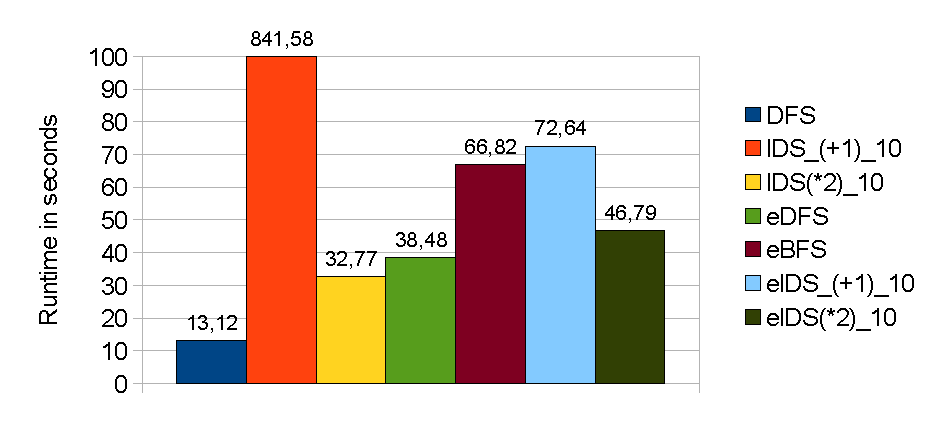
\includegraphics[width=11cm]{gfx/permsort}
\end{center}
\todo{Interpretation}
\end{frame}

\begin{frame}[fragile]%-------------------------------------------------------
\frametitle{Benchmark: Unification}
Program: Compute the last element of a list by unification
\begin{center}
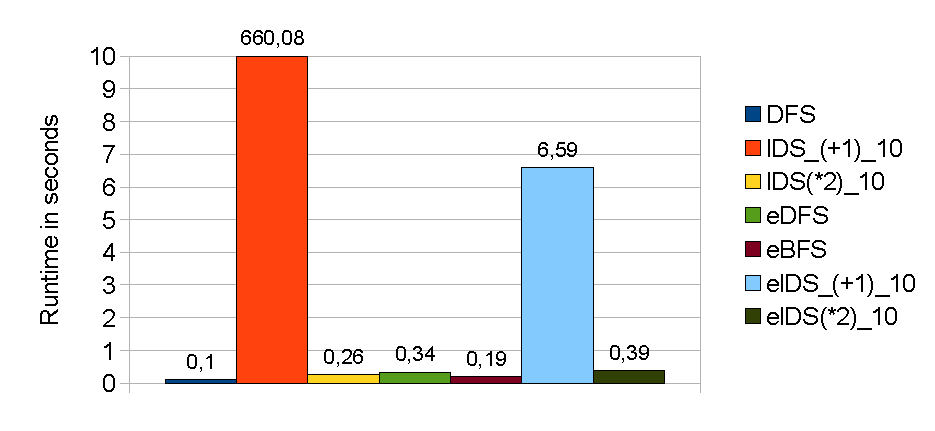
\includegraphics[width=11cm]{gfx/last}
\end{center}
\todo{Interpretation}
\end{frame}

\begin{frame}[fragile]%-------------------------------------------------------
\frametitle{Benchmark: Halve a Peano Number}
Program: halve a Peano number by inverting addition
\begin{center}
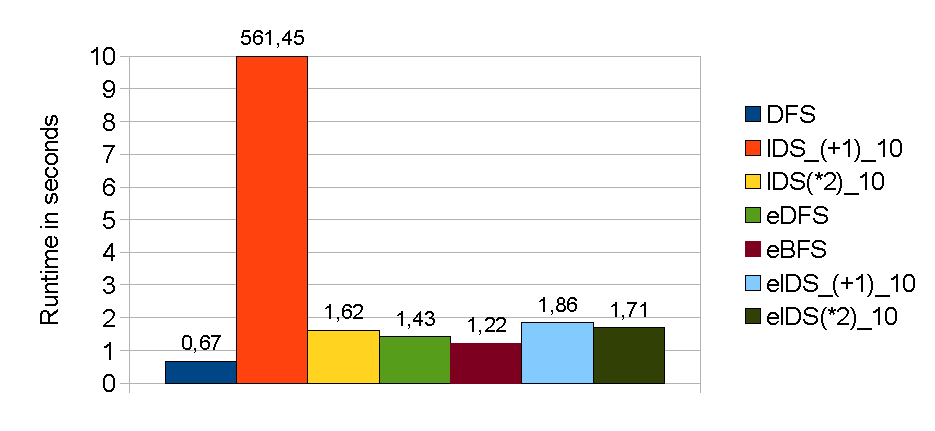
\includegraphics[width=11cm]{gfx/half}
\end{center}
\todo{Interpretation}
\end{frame}

%%%%%%%%%%%%%%%%%%%%%%%%%%%%%%%%%%%%%%%%%%%%%%%%%%%%%%%%%%%%%%%%%%%%%%%%%%%%%%

\begin{frame}[fragile]%-------------------------------------------------------
\frametitle{Set Functions}

\begin{itemize}
  \item Encapsulated search allows for searching non-determinism
        in an expression
  \item \emph{Set functions} allow to preserve non-determinism of the
        arguments, but searches for that introduced by the function
\end{itemize}

\begin{example}[Set Functions]
\begin{program}
> \textsl{set_1 f bool}
[True,False]
[False,True]
\end{program}
\end{example}

\end{frame}

\begin{frame}[fragile]%-------------------------------------------------------
\frametitle{Implementation of Set Functions}

\begin{itemize}
  \item \code{ID}s can be covered to preserve non-determinism
  \item Target structure of search needs to distinguish covered and uncovered
        non-determinism
  \item[\ergo] \code{MonadPlus} is no longer sufficient
\end{itemize}

\begin{haskell}[Covered \code{ID}s]
data ID = -- as before
        | Covered ID
\end{haskell}

\begin{haskell}[\code{MonadSearch}]
class MonadPlus m => MonadSearch m where
  splus :: ID -> m a -> m a -> m a -- preserve binary Choice
  ssum  :: ID -> [m a] -> m a      -- preserve n-ary  Choice
\end{haskell}

\end{frame}

%%%%%%%%%%%%%%%%%%%%%%%%%%%%%%%%%%%%%%%%%%%%%%%%%%%%%%%%%%%%%%%%%%%%%%%%%%%%%%

\section{Conclusion}

\begin{frame}[fragile]%-------------------------------------------------------
\frametitle{Conclusion}

\begin{itemize}
\item More flexibility
      \begin{itemize}
        \item Multiple search strategies
        \item Multiple levels to search non-determinism
      \end{itemize}
\item Applicability
      \begin{itemize}
        \item More than \code{read-eval-print} loop
        \item Non-determinism and I/O can be clearly separated
      \end{itemize}
\end{itemize}
\end{frame}

\end{document}
